\documentclass[aspectratio=169,12pt]{beamer}
\usepackage[T1]{fontenc}
\usepackage{lmodern}
\usepackage{booktabs,tabularx,listings,tikz,pgfplots,pgfpages}
\usetikzlibrary{arrows.meta,positioning}
\pgfplotsset{compat=1.18}
\definecolor{Navy}{HTML}{152B43}
\definecolor{Teal}{HTML}{007F86}
\definecolor{Coral}{HTML}{CB593E}
\definecolor{Muted}{HTML}{526476}
\definecolor{Light}{HTML}{F0F5F7}
\setbeamercolor{normal text}{fg=Navy,bg=white}
\setbeamercolor{structure}{fg=Teal}
\setbeamercolor{frametitle}{fg=Navy,bg=white}
\setbeamercolor{title}{fg=Navy}
\setbeamercolor{subtitle}{fg=Teal}
\setbeamercolor{block title}{fg=white,bg=Teal}
\setbeamercolor{block body}{fg=Navy,bg=Light}
\setbeamercolor{alerted text}{fg=Coral}
\setbeamerfont{title}{size=\LARGE,series=\bfseries}
\setbeamerfont{frametitle}{size=\Large,series=\bfseries}
\setbeamerfont{subtitle}{size=\large}
\setbeamersize{text margin left=8mm,text margin right=8mm}
\setbeamertemplate{navigation symbols}{}
\setbeamertemplate{itemize item}{\small\raise.15ex\hbox{\textbullet}}
\setbeamertemplate{itemize subitem}{\textendash}
\setbeamertemplate{frametitle}{\vspace{3mm}\insertframetitle\par\vspace{1mm}\textcolor{Teal}{\rule{\textwidth}{.7pt}}}
\setbeamertemplate{footline}{\hspace{8mm}\raisebox{2mm}{\scriptsize\textcolor{Muted}{NES security\quad|\quad\insertsectionhead}}\hfill\raisebox{2mm}{\scriptsize\insertframenumber}\hspace{8mm}}
\newcommand{\source}[1]{\par\vspace{2mm}{\tiny\color{Muted}Source: supplied paper, #1.}}
\newcommand{\takeaway}[1]{\begin{block}{Takeaway}#1\end{block}}
\newcommand{\metric}[2]{{\color{Teal}\LARGE\bfseries #1}\par\smallskip{\small #2}}
\lstset{basicstyle=\ttfamily\small,backgroundcolor=\color{Light},frame=single,rulecolor=\color{Light},breaklines=true,columns=fullflexible,showstringspaces=false,keywordstyle=\color{Teal}\bfseries,commentstyle=\color{Muted},stringstyle=\color{Coral},aboveskip=5pt,belowskip=5pt}
\pgfplotsset{nesbars/.style={ybar,bar width=14pt,ymin=0,ymax=110,ytick={0,25,50,75,100},ylabel={Failure rate (\%)},height=4.6cm,width=\textwidth,axis lines*=left,ymajorgrids=true,grid style={gray!15},tick label style={font=\scriptsize},label style={font=\small},nodes near coords,nodes near coords style={font=\tiny},legend style={font=\scriptsize,draw=none,at={(.5,1.12)},anchor=south,legend columns=2},enlarge x limits=.12}}

\title[Tab, Tab, Bug]{``Tab, Tab, Bug''}
\subtitle{Security Pitfalls of Next Edit Suggestions\\in AI-Integrated IDEs}
\author[Y. Lyu, Y. Tang, P. Chen, T. Dong, X. Wang, Z. Dong, H. Chen]{Yunlong Lyu\textsuperscript{*} \and Yixuan Tang\textsuperscript{*} \and Peng Chen \and Tian Dong\\Xinyu Wang \and Zhiqiang Dong \and Hao Chen}
\institute{The University of Hong Kong \quad McGill University \quad Independent Researchers}
\date{NES security study}
% Set \shownotestrue to generate a separate speaker-notes PDF.
\newif\ifshownotes
\shownotesfalse
\ifshownotes\setbeameroption{show notes}\else\setbeameroption{hide notes}\fi
\begin{document}
\rmfamily
\begin{frame}
\titlepage
\vspace{-4mm}
\begin{center}\footnotesize\textsuperscript{*}Equal contribution.\end{center}
\note{This presentation summarizes the supplied 18-page paper. Publication metadata in that PDF contains placeholders, so no venue or publication year is asserted here.}
\end{frame}
\begin{frame}{The talk at a glance}
\begin{columns}[T]
\column{.49\textwidth}
\textbf{Understand the mechanism}\par\medskip
1. What is NES?\\[5pt]
2. Problem statement and motivation\\[5pt]
3. Related work and the gap\\[5pt]
4. Taxonomy
\column{.49\textwidth}
\textbf{Security Evaluation}\par\medskip
5. White-box evaluation\\[5pt]
6. Black-box evaluation\\[5pt]
7. User study\\[5pt]
8. Results and findings\\[5pt]
9. Conclusions
\end{columns}
\end{frame}
\section{What is NES?}
\begin{frame}{NES predicts the next edit, including where it belongs}
\begin{block}{Next Edit Suggestions (NES)}
An IDE continuously uses recent interactions and project context to infer the developer's intent and proactively suggest the next code modification.
\end{block}
\medskip
\small
\begin{tabularx}{\textwidth}{@{}p{3.1cm}XX@{}}
\toprule
 & \textbf{Conventional completion} & \textbf{NES}\\\midrule
Primary signal & Local code near the cursor & Edit stream plus broader project context\\[5pt]
Suggested change & Continuation at the cursor & Insertions, deletions, replacements; potentially other locations or files\\[5pt]
Interaction & Complete the current line & Review, navigate, accept; repeat with Tab\\\bottomrule
\end{tabularx}
\source{Sections 1--2}
\note{Use the paper's distinction as a conceptual comparison. Implementations vary; modern completion tools may also retrieve repository context. NES is distinguished here by proactive next-edit prediction and the repeated per-edit acceptance loop.}
\end{frame}

\begin{frame}{Inside the context-to-edit pipeline}
\centering
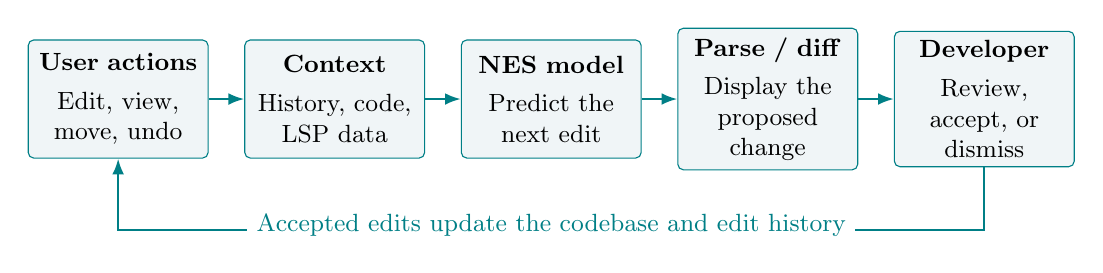
\begin{tikzpicture}[
 stage/.style={draw=Teal,fill=Light,rounded corners=2pt,text width=2.05cm,minimum height=1.5cm,align=center,font=\small},
 flow/.style={-{Latex[length=2mm]},thick,Teal}]
\node[stage] (actions) at (0,0) {\textbf{User actions}\\[3pt]Edit, view, move, undo};
\node[stage] (context) at (2.75,0) {\textbf{Context}\\[3pt]History, code, LSP data};
\node[stage] (model) at (5.5,0) {\textbf{NES model}\\[3pt]Predict the next edit};
\node[stage] (diff) at (8.25,0) {\textbf{Parse / diff}\\[3pt]Display the proposed change};
\node[stage] (accept) at (11,0) {\textbf{Developer}\\[3pt]Review, accept, or dismiss};
\draw[flow] (actions) -- (context);
\draw[flow] (context) -- (model);
\draw[flow] (model) -- (diff);
\draw[flow] (diff) -- (accept);
\draw[flow] (accept.south) -- ++(0,-.8) -| (actions.south);
\node[fill=white,text=Teal,font=\small] at (5.5,-1.6) {Accepted edits update the codebase and edit history};
\end{tikzpicture}
\takeaway{The security boundary spans \textbf{triggers, retrieved context, predicted edits, and acceptance}.}
\source{Section 2, Figure 1; simplified architectural redraw}
\note{Walk from the developer's action to event monitoring, context assembly, model prediction, response parsing and Tab acceptance. Acceptance itself becomes another edit in the history, closing the feedback loop.}
\end{frame}

\section{Problem statement and motivation}
\begin{frame}{Productive editing can silently expand security exposure}
\begin{enumerate}
\item \textbf{Implicit retrieval:} secrets or unsafe patterns enter the model's context through viewed code, history, or dependencies.
\item \textbf{Semantic changes:} a refactor can preserve functionality while losing authorization, confidentiality, or parser protections.
\item \textbf{Low-friction acceptance:} multi-location suggestions make complete security review harder during a Tab-by-Tab flow.
\end{enumerate}
\takeaway{Assessing the generated snippet alone misses risks created by the IDE workflow.}
\source{Sections 1--2}
\note{The introduction describes a reported secret-key incident involving recently viewed context and indexing exclusions. The deck focuses on the mechanism rather than asserting present-day product behavior.}
\end{frame}

\section{Related work and the gap}
\begin{frame}{Prior work establishes insecurity, poisoning, and human factors}
\begin{itemize}
\item \textbf{Generated-code security}
  \begin{itemize}
  \item \small Pearce et al. (2022); Khoury et al. (2023): insecure implementations and defaults.
  \end{itemize}
\item \textbf{Developer interaction}
  \begin{itemize}
  \item \small Perry et al. (2023); Sandoval et al. (2023): trust, prompting, and verification affect security.
  \end{itemize}
\item \textbf{Adversarial manipulation}
  \begin{itemize}
  \item \small Schuster et al. (2021); Oh et al. (2024): poisoning can steer assistants toward unsafe output.
  \end{itemize}
\end{itemize}
\medskip
\textbf{Gap:} NES implicitly collects an ongoing edit stream and proactively proposes changes. This study connects these mechanisms to security failures.
\source{Sections 1 and 7; references [27, 37, 43--46]}
\note{These are strands of prior work, not claims that all earlier assistants use only local context. Summaries follow the supplied paper's related-work discussion. Selected references are available in the optional backup slides.}
\end{frame}

\section{Taxonomy}
\begin{frame}{Taxonomy: C1, context contamination (V1--V6)}
\small
\begin{tabularx}{\textwidth}{@{}p{.7cm}p{3.7cm}X@{}}
\toprule
 & \textbf{Risk vector} & \textbf{Failure manifestation}\\\midrule
V1 & Pre-trained model & Suggest weak cryptographic primitives without a contaminated input.\\[5pt]
V2 & Recently viewed code & Reproduce a secret from a viewed configuration file.\\[5pt]
V3 & Edit history & Copy unsafe SQL concatenation from recent edits.\\[5pt]
V4 & Undo operation & Reintroduce a credential the developer removed.\\[5pt]
V5 & Structural context & Use an unsafe API without preserving local security constraints.\\[5pt]
V6 & Cross-file dependencies & Carry insecure testing patterns into production code.\\\bottomrule
\end{tabularx}
\source{Table 1; Section 3.1.1}
\note{V1 serves as the model-inherited baseline within the paper's C1 grouping. File outline and diagnostics are context inputs but are not treated as independent vectors in this taxonomy. V6's evaluation narrative uses test-to-production path handling; the appendix detection table describes a credential variant.}
\end{frame}

\begin{frame}{Taxonomy: transactional edits and human--IDE interaction}
\small
\begin{tabularx}{\textwidth}{@{}p{.7cm}p{3.9cm}X@{}}
\toprule
 & \textbf{Risk vector} & \textbf{Failure manifestation}\\\midrule
V7 & Variable logging & Copy a logging pattern onto sensitive variables.\\[5pt]
V8 & Visibility refactoring & Expose internal sensitive methods as endpoints.\\[5pt]
V9 & Component replacement & Omit parser-specific XXE protections after migration.\\\midrule
V10 & Location jumping & Skip intermediate vulnerable sites during remediation.\\[5pt]
V11 & No-Op edit & Stop suggesting before the entire fix is complete.\\[5pt]
V12 & Sequential edits & Introduce an insecure suggestion after a correct streak.\\\bottomrule
\end{tabularx}
\source{Table 1; Sections 3.1.2--3.1.3}
\note{C3 technical tests simulate an editing flow. They identify risky suggestions and incomplete remediation; they do not directly measure a human's acceptance probability. The subsequent survey provides complementary self-reported evidence.}
\end{frame}

\section{White-box evaluation}
\begin{frame}{White-box design: control the context, inspect the resulting edit}
\begin{enumerate}
\item Scan the top \textbf{1,000 Java-only GitHub projects} with CodeQL for representative insecure patterns.
\item Build a safe but incomplete target at the cursor; retain surrounding artifacts as potential propagation sources.
\item Reconstruct NES prompts using \textbf{tree-sitter}, structural context, dependencies, and synthetic edit history.
\item Query \textbf{Zeta}, apply the suggested edit, and check whether the targeted risk manifests.
\end{enumerate}
\medskip
\textbf{Scale:} 410 base cases across 9 CWE categories; 10 repetitions per case, yielding 4,100 runs.
\source{Sections 3.1 and 4; Table 2}
\note{For context propagation, keep a benign target and vary peripheral context. For transactions, initiate an opening edit and inspect the sequence. Contamination comes from artifacts within the same codebase; no external attacker is required. Eleven vectors have ten base cases each; component replacement V9 has 300. Hence 110 + 300 = 410 base cases and 4,100 repeated runs. Table 2 lists 3,000 V9 runs, unlike the other vectors' 100. The ethics appendix contains a conflicting 4,300 count; this deck follows the main evaluation table.}
\end{frame}

\begin{frame}{Security checking combines structural and semantic evidence}
\begin{columns}[T]
\column{.55\textwidth}
\begin{itemize}
\item \textbf{AST checks:} vulnerable calls or missing configuration.
\item \textbf{Regex checks:} secret literals and unsafe lexical patterns.
\item \textbf{Semantic judges:} sensitivity, data flow, or edit intent that syntax cannot resolve.
\end{itemize}
\column{.41\textwidth}
\begin{block}{LLM adjudication}
\small Five independent judges.\\[5pt]
At least \textbf{4 of 5} must flag a suggestion as insecure.\\[5pt]
\textbf{51 split-vote cases} receive manual review.
\end{block}
\end{columns}
\takeaway{Rates measure failures in deliberately activated security scenarios, rather than ordinary coding prevalence.}
\source{Section 3.1; Appendices D--E}
\note{The panel comprises DeepSeek-V3.2, Qwen3-235B-A22B, Gemini-3-Flash, Claude-Haiku-4.5, and GPT-5-mini. A 2--3 vote split is manually resolved. The detectors are useful but not a proof of exploitable behavior in every original repository.}
\end{frame}

\section{Black-box evaluation}
\begin{frame}{Black-box design: reproduce the workflow in four IDEs}
\begin{columns}[T]
\column{.44\textwidth}
\begin{block}{Systems under test}
Cursor\\GitHub Copilot\\Trae\\Zed
\end{block}
\medskip
10 cases per vector\\$12\times10=120$ selected cases\\$120\times4=480$ executions
\column{.52\textwidth}
\textbf{Manual protocol}
\begin{enumerate}
\item Open the project at the target location.
\item Recreate preparatory viewing and editing actions.
\item Trigger NES and inspect the suggestion.
\item Reload the window before the next case.
\end{enumerate}
\end{columns}
\source{Section 3.2; Appendix H}
\note{Each selected case is run once per IDE, giving ten executions per vector per IDE and forty across tools. Black-box rates move in ten-percentage-point increments per tool. This evaluation observes deployed behavior at study time; it does not assert current product behavior.}
\end{frame}

\section{User study}
\begin{frame}{User study: a survey of experience, trust, and scrutiny}
\begin{columns}[T]
\column{.5\textwidth}
\textbf{Recruitment and filtering}
\begin{itemize}
\item One multinational IT company and one U.S. university.
\item 385 responses collected; 241 professionals in the initial pool.
\item \textbf{269 retained responses} after attention-check filtering.
\end{itemize}
\column{.46\textwidth}
\textbf{Questionnaire}
\begin{itemize}
\item 12 questions covering demographics, NES usage, trust, and security perceptions.
\item Consent, anonymity, compensation, and IRB approval reported.
\item Retained cohort: 64.4\% professional; 56.9\% use NES often or always.
\end{itemize}
\end{columns}
\source{Sections 5.1--5.2; Appendices B and G}
\note{This is a self-report survey, with no observed coding task or acceptance telemetry. In the retained cohort, 59.5\% report medium-to-high NES dependence; 95.2\% use AI-integrated IDEs. The PDF's Section 5 opening is inconsistent about the analysis population; Section 5.2 and Table 3 explicitly identify the retained N=269. The professional share of this retained cohort is 64.4\%, not 241/269.}
\end{frame}

\section{Results and findings}
\begin{frame}{Reported headline rates show failures across both settings}
\begin{columns}[T]
\column{.46\textwidth}\metric{74.44\%}{White-box: Zeta\\Macro-average across 12 vectors}
\column{.46\textwidth}\metric{77.92\%}{Black-box: four IDEs\\Average across vectors and IDEs}
\end{columns}
\bigskip
\takeaway{Both Zeta and commercial IDEs frequently produce unsafe edits in the tested security scenarios.}
\smallskip
{\small These are averages across risk vectors. White-box: 4,100 runs; black-box: 480 executions.}

\source{Section 4; Table 2}
\note{Averaging the twelve reported Zeta percentages gives 74.449\%, consistent with the paper's 74.44\% headline up to rounding or truncation. Weighting the displayed rates by Table 2 run counts instead gives approximately 54.60\%. V9's 46.39\% is itself not an exact integer fraction of 3,000, so avoid claiming an exact pooled vulnerable count.}
\end{frame}

\begin{frame}{C1 results: expanded context carries unsafe patterns}
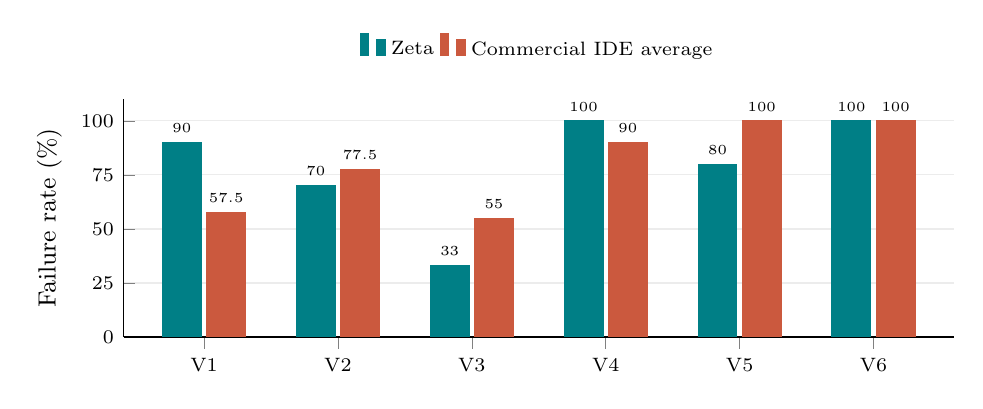
\begin{tikzpicture}
\begin{axis}[nesbars,symbolic x coords={V1,V2,V3,V4,V5,V6},xtick=data]
\addplot[fill=Teal,draw=Teal] coordinates {(V1,90)(V2,70)(V3,33)(V4,100)(V5,80)(V6,100)};
\addplot[fill=Coral,draw=Coral] coordinates {(V1,57.5)(V2,77.5)(V3,55)(V4,90)(V5,100)(V6,100)};
\legend{Zeta,Commercial IDE average}
\end{axis}
\end{tikzpicture}
\scriptsize V1 model; V2 viewed code; V3 history; V4 undo; V5 structure; V6 dependencies.\par\smallskip\small\textbf{Finding:} undo may remove a secret from the file while leaving it in model context.
\source{Table 2; Sections 4.1.1 and 4.2}
\note{Commercial systems show lower V1 failure rates, but higher failures on V2, V3 and V5. V4 and V6 remain high. These are conditional failure rates for distinct vector-specific scenarios, not controlled comparisons of interchangeable context sources.}
\end{frame}

\begin{frame}{C2 results: functional refactoring loses security invariants}
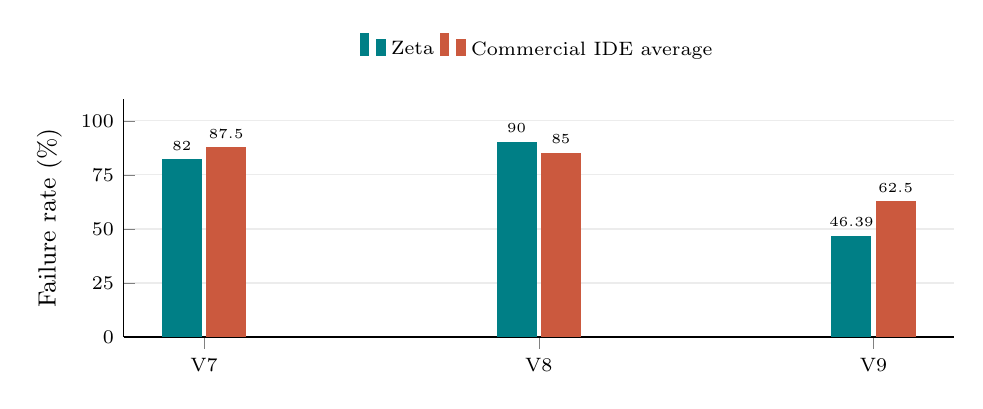
\begin{tikzpicture}
\begin{axis}[nesbars,symbolic x coords={V7,V8,V9},xtick=data]
\addplot[fill=Teal,draw=Teal] coordinates {(V7,82)(V8,90)(V9,46.39)};
\addplot[fill=Coral,draw=Coral] coordinates {(V7,87.5)(V8,85)(V9,62.5)};
\legend{Zeta,Commercial IDE average}
\end{axis}
\end{tikzpicture}
\scriptsize V7: sensitive logging; V8: endpoint exposure; V9: missing XML-parser protections.\par\smallskip\small\textbf{Finding:} functionally equivalent replacements can lose security settings.
\source{Table 2; Sections 4.1.2 and 4.2}
\note{Component replacement has much broader white-box coverage than the other two vectors. Commercial V9 is 16.11 percentage points higher than Zeta in the selected black-box cases; the scenario distributions are not identical.}
\end{frame}

\begin{frame}{C3 results: jumps, silence, and insecure later steps}
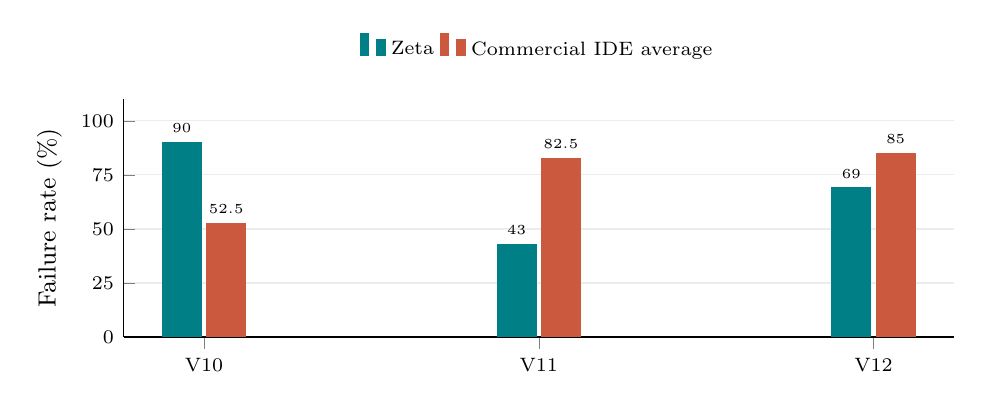
\begin{tikzpicture}
\begin{axis}[nesbars,symbolic x coords={V10,V11,V12},xtick=data]
\addplot[fill=Teal,draw=Teal] coordinates {(V10,90)(V11,43)(V12,69)};
\addplot[fill=Coral,draw=Coral] coordinates {(V10,52.5)(V11,82.5)(V12,85)};
\legend{Zeta,Commercial IDE average}
\end{axis}
\end{tikzpicture}
\scriptsize V10: location jumping; V11: No-Op edit; V12: sequential edits.\par\smallskip These are simulated workflow failures, not measured human acceptance probabilities.
\source{Table 2; Sections 3.1.3 and 4.1.3--4.2}
\note{The paper sometimes calls V12 an acceptance rate; the described technical protocol simulates developer behavior rather than observing participant acceptance. Label it as a sequence-related failure rate. The authors attribute some cross-IDE differences to debouncing, but the comparison does not causally isolate this mechanism.}
\end{frame}

\begin{frame}{Survey findings: exposure exceeds explicit security checking}
\begin{columns}[T]
\column{.31\textwidth}\metric{81.1\%}{Report encountering insecure NES suggestions}
\column{.31\textwidth}\metric{62.4\%}{Report test-to-production data suggestions}
\column{.31\textwidth}\metric{12.3\%}{Explicitly check suggestion security}
\end{columns}
\bigskip
\vspace{7mm}
\begin{itemize}
\item 28.6\% report always thoroughly reviewing NES output.
\item 32.0\% report skimming or rarely reviewing it.
\item 55.0\% select clean-looking code as a reason for acceptance.
\end{itemize}
\source{Sections 5.4--5.5; Figures 5--6; retained $N=269$}
\note{Acceptance reasons are multi-select. Review frequency and post-suggestion checking come from different questions. These self-reports establish a verification gap in this cohort, not objective vulnerability detection accuracy or a causal effect of NES on vigilance.}
\end{frame}

\begin{frame}{What limits the interpretation of these findings?}
\begin{itemize}
\item \textbf{Technical scope:} Java, one open NES model, and four commercial IDEs at study time.
\item \textbf{Sampling:} scenarios intentionally activate risks; black-box testing uses ten cases per vector per IDE.
\item \textbf{Measurement:} reconstructed prompts and hybrid detectors approximate production behavior; proprietary internals remain hidden.
\item \textbf{Human evidence:} self-reports from one company and one university; no causal acceptance experiment or population-wide estimate.
\end{itemize}
\takeaway{The study demonstrates mechanism-linked failures; everyday prevalence and mitigation effectiveness remain open questions.}
\source{Sections 3, 5, and 6}
\end{frame}

\section{Conclusions}
\begin{frame}{Security must follow the entire context-to-edit workflow}
\begin{columns}[T]
\column{.48\textwidth}
\textbf{For IDE providers}
\begin{itemize}
\item Make context sources and exclusions visible.
\item Filter suspicious context and suggestions.
\item Flag security-sensitive changes before acceptance.
\item Evaluate multi-step edits and incomplete remediation.
\end{itemize}
\column{.48\textwidth}
\textbf{For developers and teams}
\begin{itemize}
\item Treat suggested edits as unverified code.
\item Review the full transaction and skipped sites.
\item Check secrets, authorization, and migration settings explicitly.
\item Combine review, security analysis, and secure-coding training.
\end{itemize}
\end{columns}
\source{Section 6; transaction-level review follows the reported failure mechanisms}
\note{These recommendations are implications and proposed defenses, not defenses experimentally validated by this paper.}
\end{frame}

\begin{frame}{Three messages to take away}
\begin{enumerate}
\item \textbf{NES broadens the security boundary.} Ambient interactions and project context shape proactive edits.
\item \textbf{Better base models do not resolve every workflow risk.} Context propagation and lost security invariants appear across the tested systems.
\item \textbf{Review must cover the sequence.} Fluent code, navigation, or silence does not establish secure completion.
\end{enumerate}
\bigskip
\centering\Large\color{Teal}A Tab press accepts an edit;\\it does not establish its security.
\source{Sections 4--8}
\end{frame}

% Optional detailed results and references (adds two pages):
% \appendix
% \section{Backup}
\begin{frame}{Backup: complete per-vector results}
\scriptsize
\centering
\begin{tabular}{@{}llrrrrr@{}}
\toprule
 & \textbf{Vector} & \textbf{Zeta} & \textbf{Cursor} & \textbf{Copilot} & \textbf{Trae} & \textbf{Zed}\\\midrule
C1 & V1 Model & 90.00 & 40 & 50 & 90 & 50\\
 & V2 Viewed & 70.00 & 90 & 70 & 80 & 70\\
 & V3 History & 33.00 & 80 & 70 & 70 & 0\\
 & V4 Undo & 100.00 & 70 & 100 & 90 & 100\\
 & V5 Structure & 80.00 & 100 & 100 & 100 & 100\\
 & V6 Dependencies & 100.00 & 100 & 100 & 100 & 100\\\midrule
C2 & V7 Logging & 82.00 & 100 & 70 & 100 & 80\\
 & V8 Visibility & 90.00 & 100 & 100 & 70 & 70\\
 & V9 Replacement & 46.39 & 40 & 80 & 70 & 60\\\midrule
C3 & V10 Jumping & 90.00 & 40 & 60 & 40 & 70\\
 & V11 No-Op & 43.00 & 90 & 90 & 50 & 100\\
 & V12 Sequential & 69.00 & 90 & 80 & 80 & 90\\\bottomrule
\end{tabular}
\medskip\par
All entries are percentages. Zeta: 100 runs per vector except V9 (3,000).\\
Each commercial IDE: 10 executions per vector.
\source{Table 2}
\end{frame}

\begin{frame}{Backup: selected related-work references}
\scriptsize
\begin{thebibliography}{9}
\bibitem{pearce} H. Pearce et al. \emph{Asleep at the Keyboard? Assessing the Security of GitHub Copilot's Code Contributions}. IEEE S\&P, 2022.
\bibitem{khoury} R. Khoury et al. \emph{How Secure Is Code Generated by ChatGPT?} arXiv:2304.09655, 2023.
\bibitem{perry} N. Perry et al. \emph{Do Users Write More Insecure Code with AI Assistants?} ACM CCS, 2023.
\bibitem{sandoval} G. Sandoval et al. \emph{Lost at C: A User Study on the Security Implications of Large Language Model Code Assistants}. USENIX Security, 2023.
\bibitem{schuster} R. Schuster et al. \emph{You Autocomplete Me: Poisoning Vulnerabilities in Neural Code Completion}. USENIX Security, 2021.
\bibitem{oh} S. Oh et al. \emph{Poisoned ChatGPT Finds Work for Idle Hands: Exploring Developers' Coding Practices with Insecure Suggestions from Poisoned AI Models}. IEEE S\&P, 2024.
\end{thebibliography}
\source{supplied paper's bibliography; references selected for the related-work slide}
\end{frame}

\end{document}
